\def\kapitelautor{Christoph Führer}

\section{Structure of the System}
The whole structure of the system should be kept extremely simple. Simplicity was one of the major concerns we had while developing the software because the success of the application relies a lot on being intuitive and simple. Therefore it is just a sole program in a single window which gives the user a very natural feeling when using the application.

All actions performed in the background, for example creating links, database management, assigning tags, \ldots{} are not visible for the user due to the fact that it would further increase the risk of being overwhelmed by OctoTagger's functions.

\section{The final product}
After a lot of hard work we managed to finish the first version of OctoTagger. As mentioned above we made it our business to make it as intuitive as possible. That surely sounds nice but what does it actually mean?

In our case it means that the users have to understand the basic structure of the application quickly. They should be able to easily understand the main mechanics of our software so they can start using it right away. That means any difficulties that the users could experience will hinder their enjoyment and therefore would result in a loss of intuitiveness. The absolute key point on this topic was that the application has to be easy to use for the user, software has to adapt to the users, not the other way around.

To accomplish that we had the idea to make the whole program as native as possible. We wanted to give the users the impression that they are using an application which feels like it is coming directly from the operating system. They should get the experience that there is not even a third party involved. The users should get the feeling that our application is just an extension to their basic file manager, an enhancement which is easy to use and simplifies their file management.

Furthermore, we tried to design every single action that the user may take as simple as possible. Basic commands that the users know from popular programs and operating systems work exactly the same way in OctoTagger. You want to rename a file? Just press \textit{F2}. Refresh the View? Press \textit{F5}. All these classic commands that many of the users are already using by default are implemented precisely the same way in our application so there won't be any conflicts when using OctoTagger. For those not accustomed to shortcuts, there are also buttons for every action and context menus implemented.

When OctoTagger is run for the very first time this is what can be seen:

\begin{figure}[H]
    \centering
    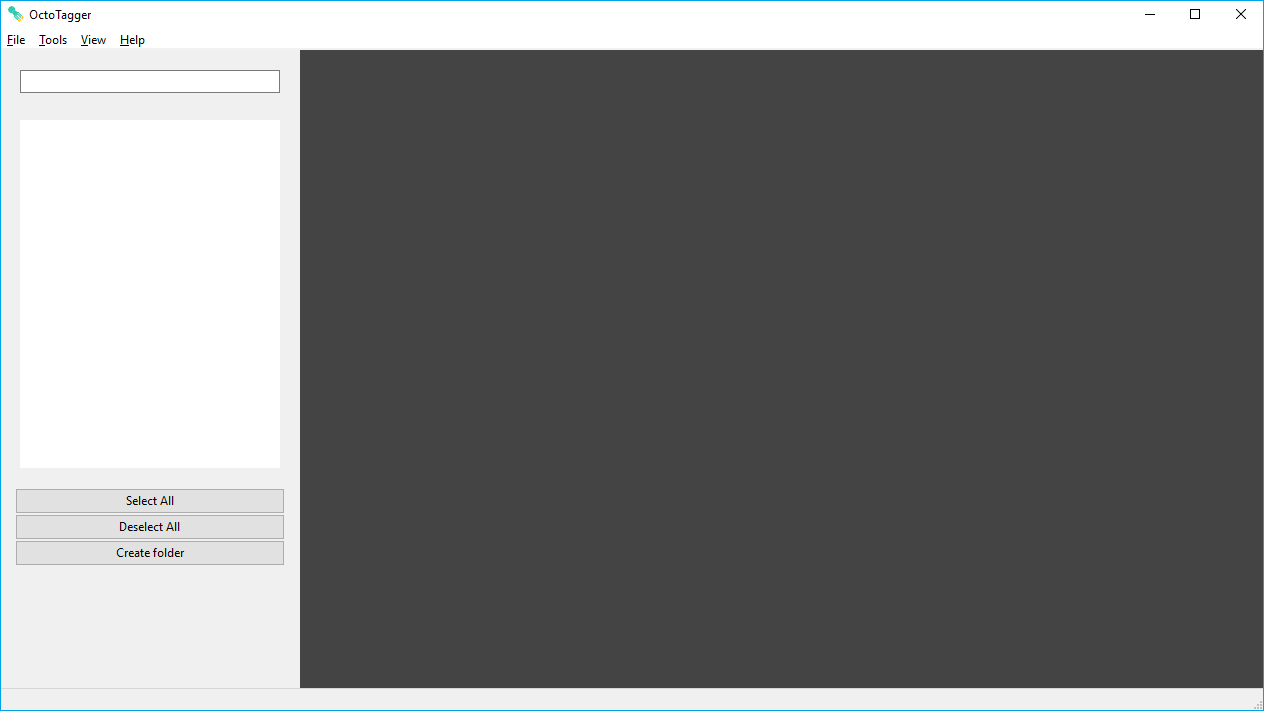
\includegraphics[width=\linewidth]{pp_04}
    \caption{The user interface at startup}
\end{figure}


At this moment it still looks pretty blank. That is because there are neither files imported nor tags assigned yet. To do so, the user has to click on the \emph{File}-Tab and then on one of the file import options.

The next step is to assign tags to the imported files. This is done by selecting the files that are to be tagged, clicking on the tag-bar in the top left corner, typing in a tag and finally pressing Enter. The files are now tagged, which can be seen in the tag-pane right below the tag-bar.
This is an example view of how your application may look like after you are done with the tagging process.

\begin{figure}[H]
    \centering
	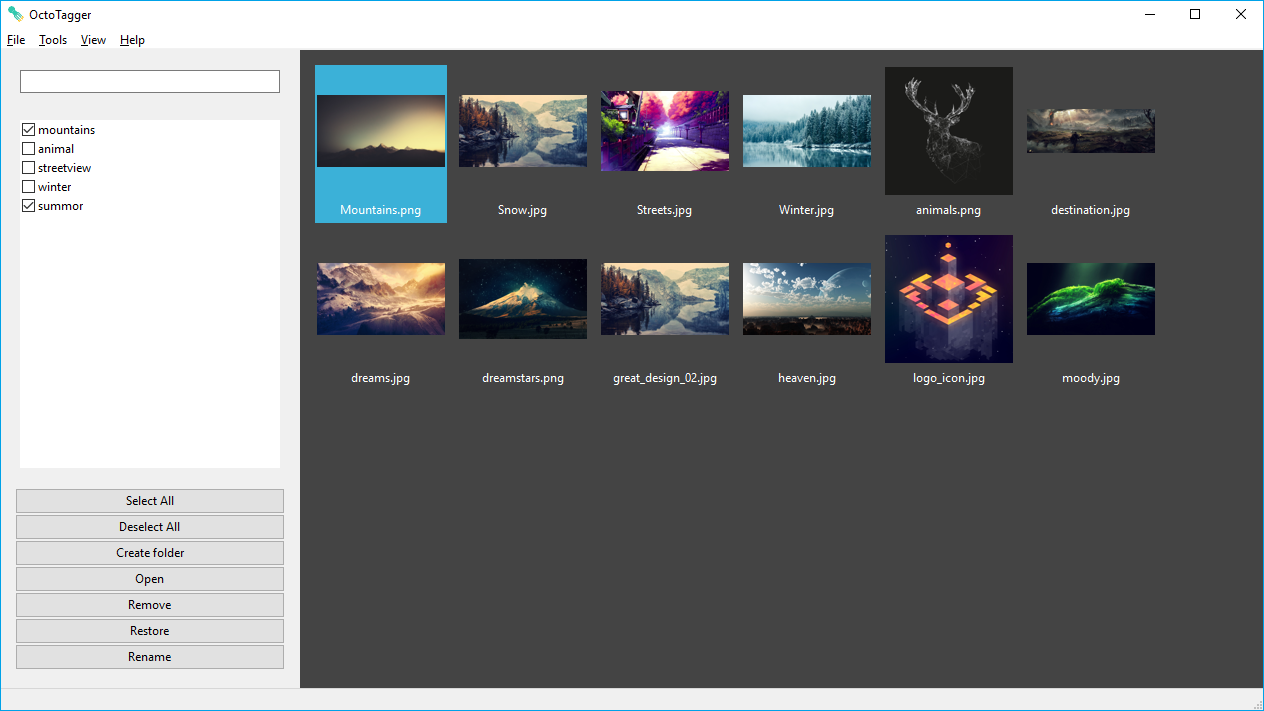
\includegraphics[width=\linewidth]{pp_03}
	\caption{User interface after importing and tagging}
\end{figure}


From this point onwards it is possible to use OctoTagger to its full extent. You can now utilize and enjoy all the different functions that are explained in the forthcoming Implementation chapter (see \cref{ch:mod:implementation}).

\subsection{Behind the scenes}
Now that an impression of the surface has been given, let's take a look at the backend. This is what your folder structure will look like right after downloading and extracting OctoTagger:

\begin{figure}[H]
    \centering
	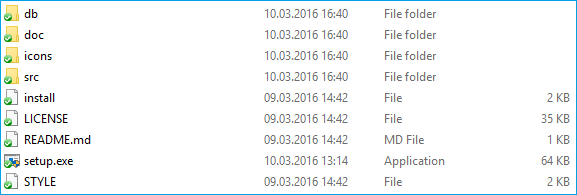
\includegraphics[width=\linewidth]{pp_06}
	\caption{File structure of OctoTagger before installing}
\end{figure}

It really is as simple as it looks. The \emph{db}-folder contains database and SQL files, in the \emph{doc}-folder is our documentation and the user manual, the source files are in the \emph{src}-folder and the \emph{icons}-folder contains logos and other images that are displayed in the application.

\section{Installation}
Installing OctoTagger is easy.

The first step after downloading and extracting the software from our website \url{http://www.octotagger.co/} would be to run the \textit{setup.exe} file on Windows, or the \emph{install} script file on Unix systems. Luckily, this is all that has to be done! Afterwards your directory will look like this:

\begin{figure}[H]
    \centering
	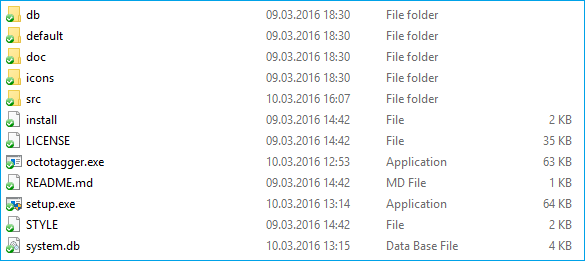
\includegraphics[width=\linewidth]{pp_05}
	\caption{File structure of OctoTagger after installing}
\end{figure}


The following things have changed:
\begin{itemize}
	\item A new folder named \emph{default} has been created. It embodies your default gallery, a \emph{files}-folder, where your imported files are saved, and a \emph{thumbnails}-folder in which the thumbnails for your imported files are saved.
	\item The file \textit{system.db} has been created
	\item An \emph{octotagger.exe} file and a shortcut on the desktop has been created (On Windows)
	\item An \emph{octotagger.desktop} file has been placed in \tfpath{\textasciitilde{}/.local/share/applications} (On Linux) 
	\item You are now able to run OctoTagger!
\end{itemize}

However, it is worth mentioning that you have to execute the setup file with administrator rights under Windows because of the simultaneously created Windows Symlink service which is also explained more in depth in the execution chapter. This is because, under Windows it is necessary to build a service which handles the link creation, due to the fact that Windows does not allow this feature without special permission. By creating a Windows service you only have to grant these rights once and are fine for as long as you keep it installed. If you want to gain a deeper understanding about this topic please consider looking at the \textit{Pywinlink} module section (see \cref{subsec:mod:pywinlink}).

\section{Goals}
We are proud to announce that all mandatory goals have been achieved! The software is running smoothly and we are all utterly satisfied with the outcome of a year of developing OctoTagger. Of course there have been some complications, challenges and other things that did not go exactly as planned, but altogether we did not have any major troubles and had a pleasant time engineering the software.

If you wish to receive more information about the goals achieved, including the optional ones, we recommend the analysis in the \textit{evaluation} chapter (see \cref{ch:mod:evaluation}). There you will also find information on how we planned the whole project in contrast to how we eventually carried it out.




















